%\todo{Pour les diff\'erences finies, faire un graphe avec sin(x), puis essayer de calculer une erreur pour la fonction de tir.
%Penser \`a le faire de mani\`ere relative en multipliant par le $x_i$. Mettre une r\'ef\'erence.}
%\todo{Ecrire une fonction \texttt{finiteDiff(fun,x,h)}.}

%---------------------------------------------------------------------------------------------------------
%---------------------------------------------------------------------------------------------------------
\section{Sur l'int\'er\^et du calcul de la jacobienne de la fonction de tir}
\label{sec:interetJac}

    On consid\`ere le probl\`eme de contr\^ole optimal suivant :
    \leqnomode
    \begin{equation}
        \tagProblem[$_\veps$]
        \left\{ 
            \begin{array}{l}
                \displaystyle J_\veps(u(\cdot))  \coloneqq \displaystyle \int_0^{t_f} \Big( \abs{u(t)}
                - \veps\, \big( \ln(\abs{u(t)}) + \ln(1-\abs{u(t)}) \,\big) \Big)
                \, \diff t\longrightarrow \min \\[1.0em]
                \dot{x}(t)                      =  \displaystyle -x(t)+u(t), \quad  \abs{u(t)} \le 1, \quad t \in \intervalleff{0}{t_f} \text{ p.p.}, \\[1.0em]
                x(0) = x_0 , \quad x(t_f) = x_f,
            \end{array}
        \right. 
        \label{eq:ocpBangReg}
    \end{equation}
    \reqnomode
    avec $\veps \in \intervalleff{0}{1}$, $t_f \coloneqq 2$, $x_0 \coloneqq 0$, $x_f \coloneqq 0.5$ et $\forall\, t \in\intervalleff{0}{t_f}$, $x(t) \in \R$.
    Notons 
    \[
        H(x,p,p^0,u) \coloneqq p \, (-x+u) + p^0\, \Big( \abs{u(t)} - \veps\, \big( \ln(\abs{u(t)}) + \ln(1-\abs{u(t)}) \,\big) \Big),
    \]
    le pseudo-hamiltonien associ\'e au probl\`eme \eqref{eq:ocpBangReg}. On consid\`ere le cas normal et on fixe $p^0 = -1$.
    La condition de maximisation du hamiltonien donne ici
    \begin{equation}
        u_\veps(p) \coloneqq 
        \left\{
        \begin{array}{cl}
            \displaystyle \frac{-2\, \veps\, \sign(p)}{\psi(p)-2\,\veps-\sqrt{\psi(p)^2+4\,\veps^2}}    & \text{ si } p\ne 0, \\[1.5em]
            \displaystyle \frac{\pm2\, \veps\,}{-1-2\,\veps-\sqrt{1+4\,\veps^2}}    & \text{ si } p=0,
        \end{array}
        \right.
        \label{eq:ocpBangRegControl}
    \end{equation}
    o\`u $\psi(p) = -1 + \abs{p}$.

    \begin{myremark}
        Dans le code on prendra
        $
            u_\veps(0) = {-2\, \veps\,}/{(-1-2\,\veps-\sqrt{1+4\,\veps^2})}.
        $
    \end{myremark}

    \begin{myExercice} Sensibilit\'e de la m\'ethode de tir et jacobienne de la fonction de tir.
        \begin{enumerate}
            \item Se rendre dans le r\'epertoire \cmd{sujet2\_jacobienne/partie1}.
            \item Impl\'ementer dans le r\'epertoire \cmd{lib} les fonctions \cmd{control}, \cmd{hvfun}, \cmd{exphvfun}, \cmd{sfun} et \cmd{ssolve},
                associ\'ees au probl\`eme \eqref{eq:ocpBangReg}.
            \item Ex\'ecuter le script \cmd{main.m} et v\'erifier les r\'esultats, \ie comparer \`a la figure \ref{fig:results_ocpBangRegControl}.
            \item V\'erifier que pour $\veps=0.01$, la m\'ethode de tir $S(y)=0$ associ\'ees au probl\`eme \eqref{eq:ocpBangReg} converge
                si l'on donne comme point de d\'epart $y^{(0)}=0.37$ ou $y^{(0)}=0.39$, mais ne converge pas pour $y^{(0)}=0.38$.
            \item V\'erifier que la m\'ethode de tir (pour $\veps=0.01$) converge si l'on donne comme point de d\'epart $y^{(0)}=0.38$, si l'on
                prend comme erreur locale d'int\'egration les valeurs $\cmd{RelTol} = \cmd{Abstol} = 1e^{-6}$ (voir \cmd{>> doc ode45}
                et \cmd{>> doc odeset}).
        \end{enumerate}
        \anoter Nous allons voir que le probl\`eme de convergence vient du calcul de la jacobienne de la fonction de tir (qui ici est calcul\'ee par
        diff\'erences finies).
    \end{myExercice}

    \begin{figure}[ht!]
        \begin{center}
            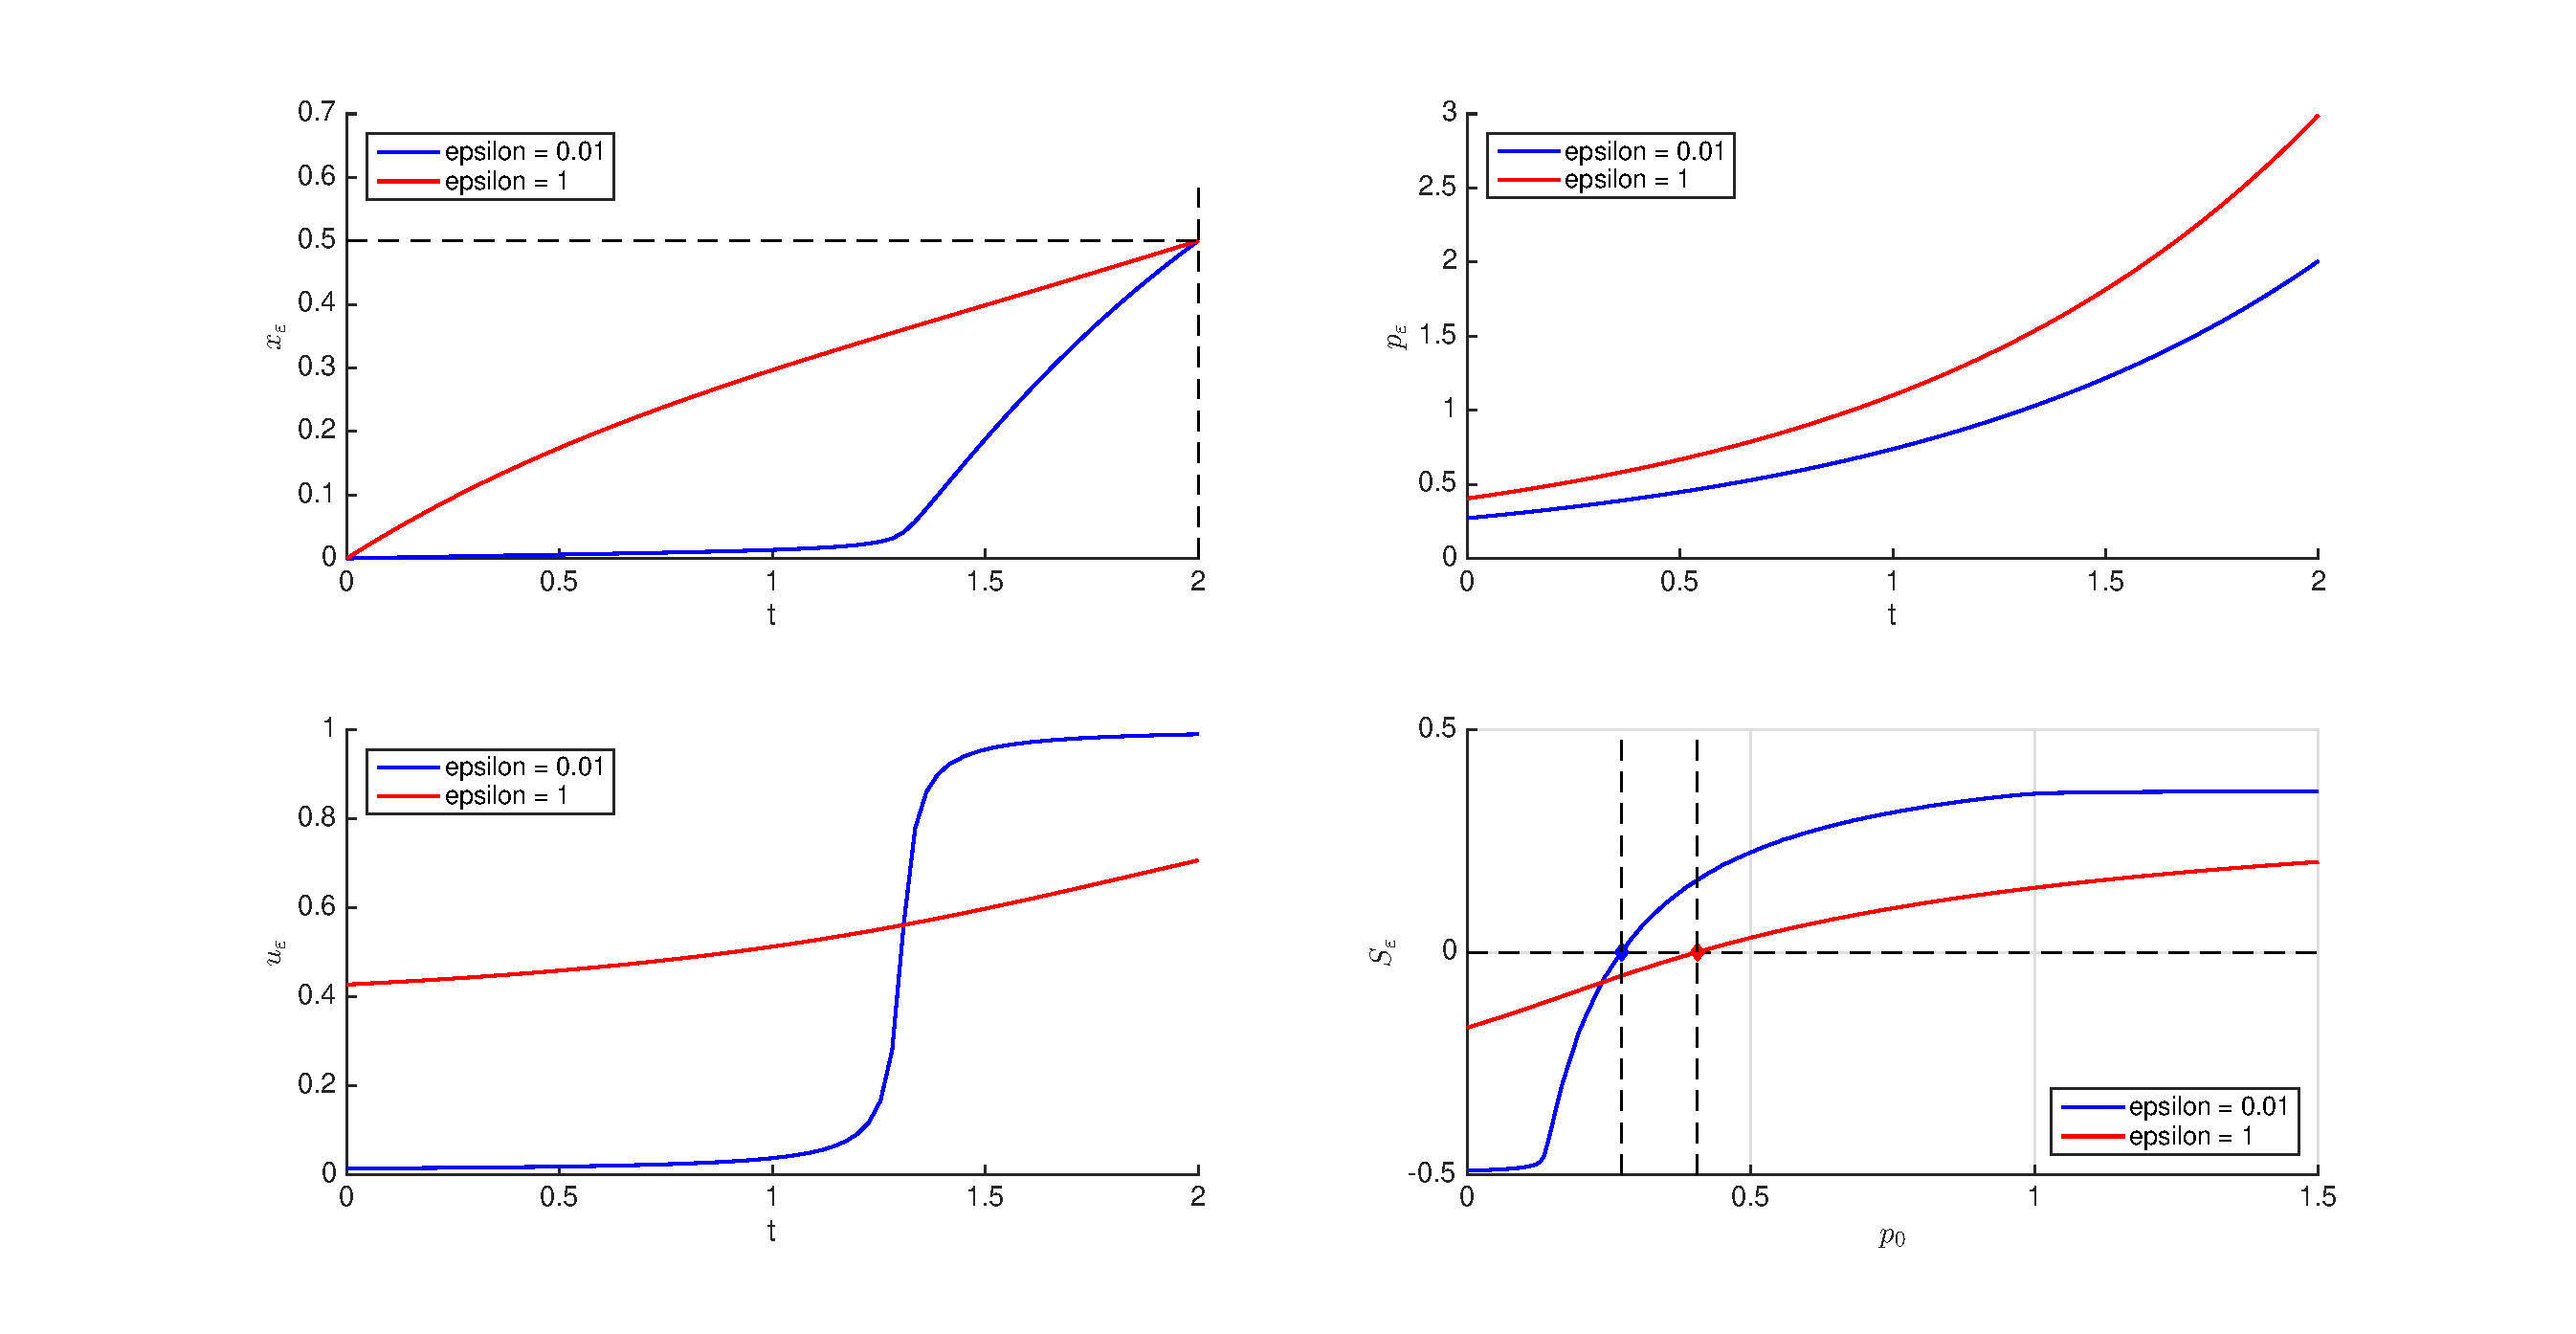
\includegraphics[width=0.99\textwidth]{results_ocpBangRegControl}
        \end{center}
        \caption{R\'esultats apr\`es ex\'ecution du fichier \cmd{sujet2\_jacobienne/partie1/main.m}.}
        \label{fig:results_ocpBangRegControl}
    \end{figure}

%---------------------------------------------------------------------------------------------------------
%---------------------------------------------------------------------------------------------------------
\section{Introduction aux diff\'erences finies}

%------------------------------------------------------------------
\subsection{Rappels}

Consid\'erons deux espaces de Banach $(E,\norme{\cdot}_E)$ et $(F,\norme{\cdot}_F)$.
Soit $g\colon E \to F$ une application. On rappelle, pour $h\in E$, la notation de Landau $\petito{h}$~:
\[
    g(h)=o(\norme{h}_E) \quad  \Longleftrightarrow  \quad \exists\, \veps \colon E \to F, \text{ tel que } g(h) = \norme{h}_E \, \veps(h) \text{ et } 
    \lim_{\norme{h}_E \to 0} \norme{\veps(h)}_F = 0.
\]

\begin{definition}[Diff\'erentielle de Fr\'echet]
    Soient une application $f\colon\Omega \subset E \to F$, $\Omega$ ouvert et un point $x\in \Omega$.
    On dit que $f$ est \emph{diff\'erentiable} au point $x$ ssi il existe une application $T_{f,x} \in \Lcal(E,F)$ telle que 
    pour tout $h\in E$ v\'erifiant $x+h\in\Omega$, on ait
    \[
        f(x+h)-f(x) - T_{f,x}(h) = o(\norme{h}_E).
    \]
    L'application lin\'eaire continue $T_{f,x}$, si elle existe est unique, et on l'appelle la \emph{diff\'erentielle de Fr\'echet} de $f$ au point $x$.
\end{definition}

\begin{myremark}
    On utilisera la notation $\diff f(x) \cdot h \coloneqq T_{f,x}(h)$ ou $f'(x) \cdot h \coloneqq T_{f,x}(h)$.
\end{myremark}

Si $f$ est diff\'erentiable en $x$ et si $h$ est un vecteur de $E$, on a
\begin{equation*}
    \diff f(x) \cdot h = \lim_{t\to 0} \frac{f(x+t\,h)-f(x)}{t},
\end{equation*}
$t$ \'etant une variable r\'eelle. Ainsi, $\diff f(x) \cdot h$ est \'egal au vecteur vitesse $\frac{\diff}{\diff t} f(x+t\,h)|_{t=0}$,
appel\'ee \emph{d\'eriv\'ee directionnelle} de $f$ en $x$ dans la direction $h$.

%------------------------------------------------------------------
\subsection{Diff\'erences finies}

Soient $f$ une fonction lisse de $\R^n$ dans $\R^m$, $x$ un point de $\R^n$ et $h$ un vecteur de $\R^n$. On note $g \colon t \mapsto f(x+t\,h)$.
Pour $t$ proche de $0$, on a d'apr\`es la formule de Taylor-Young~:
\begin{equation*}
    g(t) = \sum_{k=0}^n \frac{t^k}{k!}\, g^{(k)}(0) + R_n(t), \quad R_n(t) = o(t^n),
\end{equation*}
et d'apr\`es l'in\'egalit\'e de Taylor-Lagrange,
\begin{equation*}
    \abs{R_n(t)} \le \frac{M_n\, \abs{t}^{n+1}}{(n+1)!},
\end{equation*}
o\`u $M_n$ est une constante positive majorant la d\'eriv\'ee \`a l'ordre $n+1$.
De m\^eme,
\begin{equation*}
    g(-t) = \sum_{k=0}^n \frac{(-t)^k}{k!}\, g^{(k)}(0) + o(t^n).
\end{equation*}

\paragraph*{Formule des diff\'erences finies avants.} La m\'ethode des diff\'erences finies avants consiste \`a approcher la diff\'erentielle de 
$f$ en $x$ dans la direction de $h$ par la formule suivante~:
\begin{equation}
    \frac{f(x+t\,h)-f(x)}{t} = \frac{g(t)-g(0)}{t} = g'(0) + \frac{t}{2}\, g''(0) + \frac{t^2}{3!}\, g^{(3)}(0) + o(t^2).
    \label{eq:diffFinieAvant}
\end{equation}
On obtient ainsi une approximation de $g'(0) = \diff f(x) \cdot h$ \empha{d'ordre 1} si $g''(0) \ne 0$ ou au moins d'ordre 2 sinon.
%
Notons $\comp(g,t)$ la valeur $g(t)$ calcul\'ee num\'eriquement et supposons que l'on puisse major\'ee l'erreur relative du calcul num\'erique par~:
\[
    \abs{\comp(g,t) - g(t)} \le \theta L_f,
\]
o\`u $L_f$ est une borne de la valeur de $g(\cdot)$ sur le domaine d'int\'er\^et. Ainsi, pour $t>0$ petit, on a~:
\begin{equation*}
    \begin{aligned}
        \absStyle{\frac{\comp(g,t) - \comp(g,0)}{t} - g'(0)}  & = \absStyle{\frac{g(t) + e_1 - g(0) - e_2}{t} - g'(0)} \\
        & = \absStyle{\frac{R_1(t)}{t} + \frac{e_1-e_2}{t}} \\
        & \le \frac{M_1\, t}{2} + 2 \frac{\theta L_f}{t} \eqqcolon \phi(t).
    \end{aligned}
\end{equation*}
La fonction $\phi$ atteint son minimum en la valeur
\[
    \tsol = 2 \sqrt{\frac{\theta L_f}{M_1}},
\]
et si on suppose que le ratio $L_f / M_1$ est d'un ordre de grandeur peu \'elev\'e, alors le choix suivant pour $t$ est presque optimal~:
\[
    \tsol = \sqrt{\theta },
\]
et on obtient ainsi une approximation de l'erreur totale $\phi(\tsol)$ proportionnelle \`a $\sqrt{\theta}$.

\paragraph*{Formule des diff\'erences finies centr\'ees.} La m\'ethode des diff\'erences finies centr\'ees consiste \`a approcher la diff\'erentielle de 
$f$ en $x$ dans la direction de $h$ par la formule suivante~:
\begin{equation}
    \frac{f(x+t\,h)-f(x-t\,h)}{2\,t} = \frac{g(t)-g(-t)}{2\,t} = g'(0) + \frac{t^2}{3!}\, g^{(3)}(0) + \frac{t^4}{5!}\, g^{(5)}(0) + o(t^4).
    \label{eq:diffFinieAvant}
\end{equation}
On obtient ainsi une approximation de $g'(0) = \diff f(x) \cdot h$ \empha{d'ordre 2} si $g^{(3)}(0) \ne 0$ ou au moins d'ordre 4 sinon.

\begin{myremark}
    \anoter Les diff\'erences finies centr\'ees sont d'ordre plus \'elev\'e mais demandent plus d'\'evaluations de la fonction $f$.
    %d\`es lors que l'on 
    %cherche \`a calculer la d\'eriv\'ee directionnelle de $f$ dans plusieurs directions, par exemple pour le calcul de la jacobienne de $f$ avec $n>1$.
\end{myremark}

\begin{myQuestion}
    \label{question:diff_finies}
    Sachant que l'on commet une erreur num\'erique lors du calcul de $g$ en un point $t$, quel est le choix optimal pour $t$ pour approcher la valeur de $g'(0)$ 
    par diff\'erences finies centr\'ees ? Quelle est alors la valeur de la borne de l'erreur totale ?
\end{myQuestion}

\begin{myExercice} Approximation par diff\'erences finies avants.
    \begin{enumerate}
        \item Se rendre dans le r\'epertoire \cmd{sujet2\_jacobienne/partie2}.
        \item Impl\'ementer la fonction \cmd{finiteDiff} dans le fichier \'eponyme du r\'epertoire \cmd{lib},
            qui approche par diff\'erences finies avants, la d\'eriv\'ee
            directionnelle de $f$ en $x$ dans la direction $h$.
        \item Ex\'ecuter le script \cmd{mainTestFD.m} et v\'erifier que la valeur optimale de $t$ est de l'ordre de $\sqrt{\veps_\mathrm{mach}}$
            o\`u $\veps_\mathrm{mach}$ est l'epsilon machine. Ici, $f(x)=-\cos(x)$.
    \end{enumerate}
\end{myExercice}

%---------------------------------------------------------------------------------------------------------
%---------------------------------------------------------------------------------------------------------
\section{Jacobienne de la fonction de tir}

%------------------------------------------------------------------
\subsection{Calcul de la jacobienne de la fonction de tir}

Voyons le calcul de la jacobienne de la fonction de tir sur un exemple.
Donnons la jacobienne de la fonction de tir associ\'ee au probl\`eme \eqref{eq:ocpBangReg}. Pour ce probl\`eme, la fonction de tir
s'\'ecrit 
\[
    S(y) = \Pi_x(z(t_f,x_0,y)) - x_f = x(t_f,x_0,y) - x_f,
\]
avec $\Pi_x$ la projection canonique $\Pi_x(x,p) = x$ et
o\`u $z(\cdot,z_0)$ est solution de $\dot{z}(t) = \vvec{H}(z(t))$, $z(0,z_0) = z_0$, avec la notation habituelle $z_0 = (x_0,p_0)$. Ainsi, on a :
\begin{equation}
    \indent \diff S(y) \cdot h = \frac{\partial x}{\partial p_0}(t_f,x_0,y) \cdot h = \frac{\partial x}{\partial z_0}(t_f,x_0,y) \cdot (0,h)
    = \Pi_x\left(\frac{\partial z}{\partial z_0}(t_f,x_0,y) \cdot (0,h) \right).
    \label{eq:sjacSimple}
\end{equation}
On voit alors que le calcul de la jacobienne de $S$ fait intervenir
\[
    \frac{\partial z}{\partial p_0}(t_f,x_0,y) = \frac{\partial z}{\partial z_0}(t_f,x_0,y) \cdot(0_n, I_n),
\]
o\`u $0_n$ est la matrice nulle de taille $n$,
$I_n$ est la matrice identit\'e, et $n$ est la dimension de l'\'etat.
Enfin, d'apr\`es le cours sur les \'equations diff\'erentielles ordinaires\footnote{J. Gergaud, \'Equations diff\'erentielles ordinaires.},
$ \frac{\partial z}{\partial p_0}(\cdot,x_0,y)$ est solution des \emph{\'equations variationnelles} suivantes~:
\begin{equation}
    \dot{\wideparen{\delta z}}(t) =  \displaystyle \diff \vvec{H}(z(t,x_0,y))\cdot \delta z(t), \quad
    \delta z(0) = \begin{bmatrix}
                    0_n \\
                    I_n
                    \end{bmatrix}.
    \label{eq:eqvar}
\end{equation}

\begin{myremark}
    Si l'on \'ecrit 
    \[
        z(t, x_0, p_0) = (x_0, p_0) + \int_0^t \vvec{H}(z(s,x_0,p_0)) \diff s,
        \]
    et si $z(\cdot, x_0, p_0)$ est d\'erivable par rapport \`a la condition initiale, alors on retrouve le r\'esultat en d\'erivant~:
    \[
        \frac{\partial z}{\partial p_0}(t,x_0,p_0) = (0_n, I_n) +
        \int_0^t \diff \vvec{H}(z(s,x_0,p_0)) \cdot \frac{\partial z}{\partial p_0}(s,x_0,p_0) \diff s.
    \]
\end{myremark}

L'objectif dans un premier temps est de retrouver les r\'esultats de la figure \ref{fig:results_jacobienne}.
\begin{figure}[ht!]
    \begin{center}
        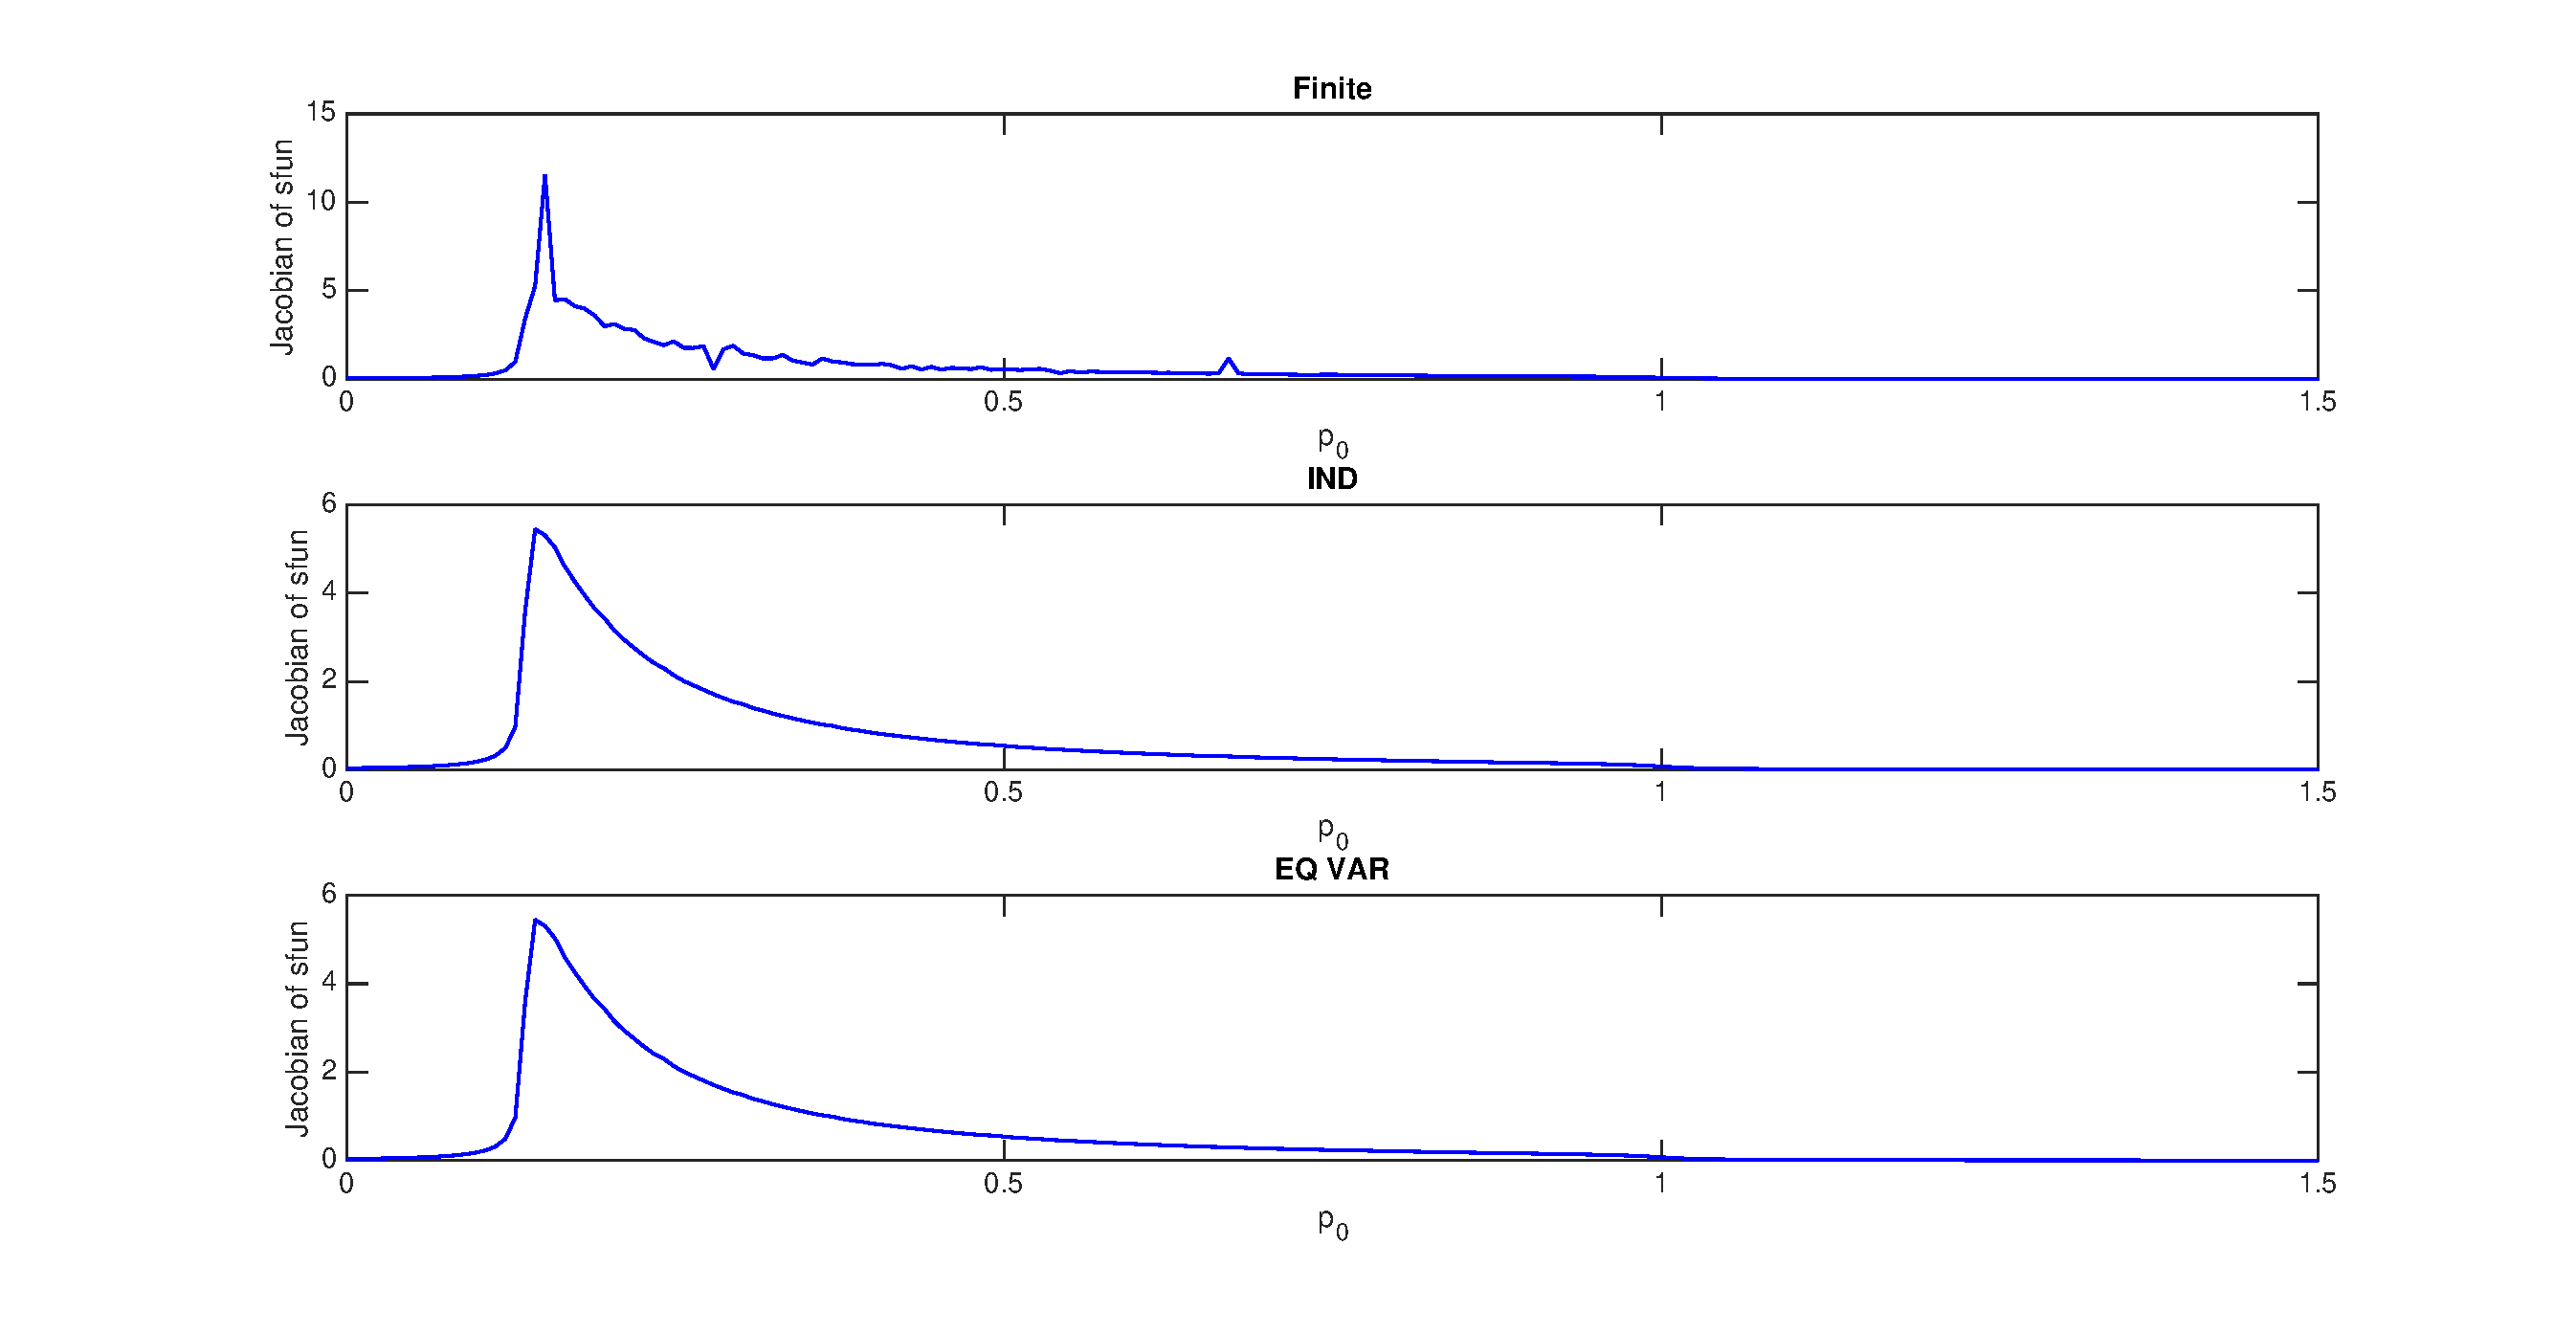
\includegraphics[width=0.99\textwidth]{results_jacobienne}
    \end{center}
    \vspace{-3em}
    \caption{R\'esultats apr\`es ex\'ecution du fichier \cmd{sujet2\_jacobienne/partie2/mainDiff.m}.}
    \label{fig:results_jacobienne}
\end{figure}

%------------------------------------------------------------------
\subsection{Diff\'erences finies (externes)}

\begin{myremark}
    Attention, la fonction \cmd{ssolve} est d\'ej\`a \'ecrite.
\end{myremark}

\begin{myExercice} Approximation de la jacobienne de la fonction de tir par diff\'erences finies.
    \begin{enumerate}
        \item Impl\'ementer dans le r\'epertoire \cmd{lib} de \cmd{sujet2\_jacobienne/partie2}, les fonctions \cmd{control}, \cmd{hvfun},
            \cmd{exphvfun}, \cmd{sfun}
                associ\'ees au probl\`eme \eqref{eq:ocpBangReg}.
        \item Utiliser la fonction \cmd{finiteDiff} pour compl\'eter la partie calcul par diff\'erences finies (\cmd{finite})
            dans le fichier \cmd{lib/sjac.m}.
        \item Ex\'ecuter le script \cmd{mainDiff.m} et v\'erifier les r\'esultats, \cf figure \ref{fig:results_jacobienne}.
    \end{enumerate}
\end{myExercice}

%------------------------------------------------------------------
\subsection{Diff\'erentiation interne de Bock}

Nous allons approcher par diff\'erence finie le deuxi\`eme membre de l'\'equation variationnelle \eqref{eq:eqvar}\footnote{%
H.G. Bock. \emph{Numerical treatment of inverse problems in chemical reaction kinetics}, in K.~H. Hebert, P.~Deuflhard, and W.~Jager, editors,
Modelling of chemical reaction systems, volume 18 of Springer series in Chem. Phys., pages 102--125, 1981.}.
On a alors, en notant $z(t) \coloneqq z(t,x_0,y)$,
\[
    \diff \vvec{H}(z(t)) \cdot \delta z(t) \approx \frac{\vvec{H}(z(t) + \eta\, \delta z(t)) - \vvec{H}(z(t))}{\eta},
\]
avec $\eta > 0$ petit. On peut prendre $\eta$ de l'ordre de la racine carr\'ee de l'epsilon machine.
\begin{myExercice} Approximation de la jacobienne de la fonction de tir par diff\'erences finies interne (de Bock).
    \begin{enumerate}
        \item Compl\'eter les parties calcul par diff\'erences finies internes (\cmd{ind}) dans les fichiers \cmd{lib/dhvfun.m} et \cmd{lib/sjac.m}.
            Utiliser la fonction \cmd{expdhvfun} qui est d\'ej\`a cod\'ee dans le fichier \cmd{lib/expdhvfun.m}.
        \item Ex\'ecuter le script \cmd{mainDiff.m} et v\'erifier les r\'esultats, \cf figure \ref{fig:results_jacobienne}.
    \end{enumerate}
\end{myExercice}

%------------------------------------------------------------------
\subsection{\'Equations variationnelles}

Nous allons directement r\'esoudre les \'equations variationnelles \eqref{eq:eqvar} pour calculer la jacobienne de la fonction de tir.
Pour cela, nous donnons pour $p\ne0$,
\[
    \displaystyle
    u'_\veps(p) = \frac{ 2\, \veps \left( 1 - \displaystyle\frac{\psi(p)}{\sqrt{\psi(p)^2+4\,\veps^2}} \right) }
    { \left( \psi(p) - 2\, \veps - \sqrt{\psi(p)^2+4\,\veps^2} \right)^2 }.
\]
Bien que la fonction ne soit pas d\'efinie pour $p=0$, et donc non d\'erivable, on prendra dans le code la m\^eme expression.
\begin{myExercice} Calcul de la jacobienne de la fonction de tir via les \'equations variationnelles.
    \begin{enumerate}
        \item Compl\'eter le fichier \cmd{lib/dcontrol.m} qui code la fonction $u'_\veps$.
        \item Compl\'eter les parties calcul via les \'equations variationnelles (\cmd{eqvar}) dans les fichiers \cmd{lib/dhvfun.m} et \cmd{lib/sjac.m}.
        \item Ex\'ecuter le script \cmd{mainDiff.m} et v\'erifier les r\'esultats, \cf figure \ref{fig:results_jacobienne}.
    \end{enumerate}
\end{myExercice}

%---------------------------------------------------------------------------------------------------------
%---------------------------------------------------------------------------------------------------------
\section{R\'esolution des \'equations de tir}

\begin{myExercice} R\'esolution des \'equations de tir : ex\'ecution du script \cmd{main.m}.
    \begin{enumerate}
        \item V\'erifier que la m\'ethode de tir ne converge pas pour $y^{(0)} = 0.38$
            avec le calcul de la jacobienne par diff\'erences finies, avec les tol\'erances
            d'int\'egration num\'erique par d\'efaut et un pas de diff\'erences finies de l'ordre de la racine carr\'ee de 
            l'epsilon machine (modifier \cmd{lib/sjac.m} si n\'ecessaire).
            On retrouve alors le comportement par d\'efaut vu en section \ref{sec:interetJac}.
        \item V\'erifier que la m\'ethode converge si l'on prend les tol\'erances par d\'efaut mais que l'on choisit un pas adapt\'e, de l'ordre
             de la racine carr\'ee de l'erreur d'int\'egration num\'erique (modifier \cmd{lib/sjac.m} si n\'ecessaire).
             On rappelle que les tol\'erances par d\'efaut donn\'ees par
             \cmd{odeset} sont $\cmd{AbsTol} = 1e^{-6}$ et $\cmd{Reltol} = 1e^{-3}$.
         \item V\'erifer que la m\'ethode (\cmd{ssolve}) converge si l'on calcule la jacobienne avec l'option \cmd{ind} ou \cmd{eqvar}.
    \end{enumerate}
\end{myExercice}


\begin{myremark}
    \anoter On peut voir sur la figure \ref{fig:extrait_doc_matlab}, le comportement de la fonction \cmd{fsolve} de \matlab\ vis \`a vis de
    l'utilisation des diff\'erences finies pour le calcul approch\'e de la jacobienne. Par d\'efaut, le pas est de l'ordre de la racine carr\'ee
    de l'epsilon machine pour les diff\'erences finies avants et de la racine cubique pour les diff\'erences centr\'ees.
\end{myremark}

\begin{figure}[ht!]
    \begin{center}
        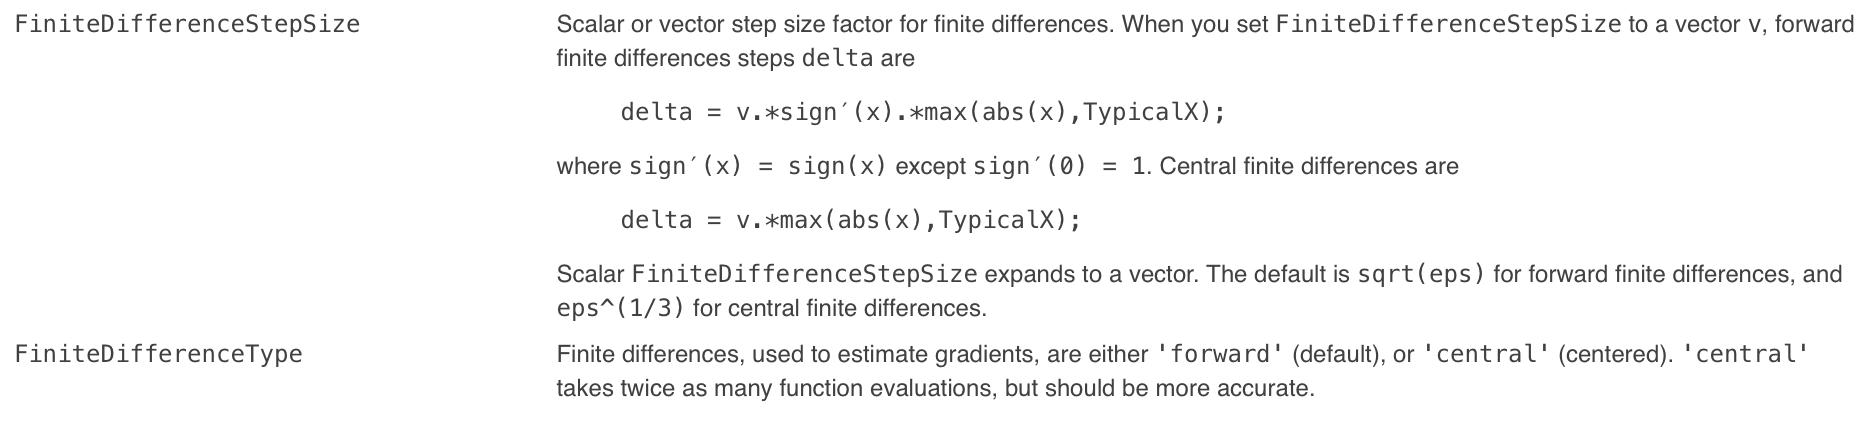
\includegraphics[width=0.99\textwidth]{matlab_finite_diff_stepsize}
    \end{center}
    \vspace{-1em}
    \caption{Extrait de la documentation de \matlab\ sur les diff\'erences finies avec \cmd{fsolve}.}
    \label{fig:extrait_doc_matlab}
\end{figure}
